\subsection{Measurement}
\subsubsection{Measurement Parameter}
\label{subsec:measurements}
To perform various measurements that reflect realistic scenarios a large web content provider will encounter, a topology consisting of several components was composed. As HTTP client machines, Amazon AWS microinstance VMs \cite{amazon} located at different geographical locations (Europe, North America and Asia) are used. Different geographical locations used on client side, ensure to perform measurements seen from different magnitudes of Round Trip Times towards the destination web server located in Amsterdam. On server side two TLS enabled webserver instances are running on one physical machnine in order to conduct measurements for both protocols - HTTP/1.1 and HTTP/2. Three reference HTML pages of different sizes and different numbers of statically linked resources have been created to be compared. These pages reflect the sizes that can be encountered in most common websites and has been derived from top 100 websites statistics \cite{httparchive}. The appropriate web page sizes including the number of resources are listed in Table \ref{table:pages}.

\begin{table}[h]
	\centering
\begin{tabular}{ | c | c | c | }

\hline
\textbf{Web Page} & \textbf{Size (kB)} & \textbf{Number of links}\\ \hline \hline
small.html &  20 & 2 \\ \hline
medium.html &  600 & 7\\ \hline 
large.html &  1600 & 54 \\
\hline
\end{tabular}
\caption{different Web Pages}
\label{table:pages}
\end{table}

So far, we have defined different static parameters that will be applied while performing the measurement. These parameters include different Round Trip Times (RTTs) and different web page sizes.  
To simulate varying and realistic load scenarios on the server, the number of clients and thereby the number of requests towards the web servers is incremented during each test starting from one client upto maximal 750 clients in parallel.
\\  
\subsubsection{Measurement Tools}
It is essential to choose and implement the right tool and method to measure the response/request times characteristics of the HTTP/1.1 and HTTP/2 protocol and to be able to compare them with each other. Thus, the benchmarking tool was chosen carefully and with respect to retrieve accurate measurement data that can be used to compare both HTTP versions with each other. 
H2load \cite{h2load} was elected as the best candidate for that purpose. It has been developed to run benchmarking tests against HTTP/2 enabled web servers. 
It can also be used to conduct measurements against HTTP/1.1 enabled web servers if, like in that case, a HTTP/2 - HTTP/1.1 reverse proxy is used that is capable to translate HTTP/2 requests into HTTP/1.1 requests on server side. 
It is possible to start h2load with a file option, that includes a list of URIs that each measurement will request in parallel. H2load returns after each measurement round accurate and valuable data, like the retrieved  amount of header and body data in bytes per request. Furthermore it returns the minimum, maximum and mean round trip time for each web page request and the actual performance in requests/second. 
\\
\subsubsection{Measurement Methods}
In order to collect statistical analysable data, all measurements are performed with twenty repetitions. A wrapper script was created that performs the measurements using h2load, does mean calculations on the data and writes them into a file. The data is later processed for visualizing round trip times and other measurements. The wrapper script can be found at the end of that report as part of the appendices. 
\\
It is important to notice that the main difference between HTTP/1.1 and HTTP/2 sessions is based on the number of created TCP sessions on server side. A HTTP/1.1 client (e.g. web browser) opens for each HTML link that is present in a HTML web page a separate TCP session to the web server. In contrast to HTTP/1.1, the new HTTP/2 protocol opens one single TCP session towards the server and multiplexes all requested data over multiple streams within a single TCP session. Thus, the maximum number of concurrent streams for each HTTP/2 session is set equal to the amount of requested URIs in all measurements. Figure \ref{fig:httpwatch} shows HTTP/1.1 GET requests in order to get the entire set of resources the reference web page (large.html) includes.


\begin{figure}[H]
	\centering
	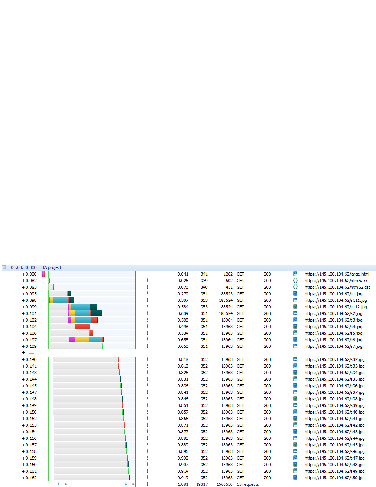
\includegraphics[scale=2,trim=0.0cm .0cm .0cm 4.5cm,clip]{images/http.pdf}
	\caption{HTTP/1.1 GET requests for large.html}
	\label{fig:httpwatch}
\end{figure}

HTTP/2 handles all GET requests in a single TCP connection by using multiple streams \textit{s}, thus the expected number of TCP connections \textit{t} will be equal to the number of concurrent simulated clients \textit{n}. For HTTP/1.1  we expect the number of TCP connection \textit{t} as a function of the product of concurrent clients \textit{n} by the requested number of HTML links \textit{l}. Thus we can describe the number of TCP sessions for HTTP/1.1 as \begin{equation}
t=f(n)=n*l \qquad \text{and} \qquad l \geq 1\end{equation} and for HTTP/2 as \begin{equation} t=f(n)=n \qquad \text{and} \qquad s=l; l\geq 1; s \in n \end{equation}

That results in Table \ref{table:tcpconnects} which shows the expected numbers of TCP connections towards the web server during some stages in the measurements with an assumed number of \textit{l=55} HTML links per page request.

\begin{table}[h]
	\centering
\begin{tabular}{ | c | c | c | }

\hline
\textbf{clients/requests \textit{n}} &\textbf{\textit{t} (HTTP/2)} &\textbf{\textit{t} (HTTP/1.1)}\\ \hline \hline
1 & 1 & 55 \\ \hline
10 & 10 & 550\\ \hline
50 & 50 & 2750\\ \hline
150 & 150 & 8250\\ \hline
300 & 300 & 16500 \\ \hline
500 & 500 & 27500\\ \hline 
750 & 750 & 41250\\
\hline
\end{tabular}
\caption{Number of TCP connections HTTP/1.1 and HTTP/2}
\label{table:tcpconnects}
\end{table} 